%\input{preamble}

%\begin{document}
\section{Standard Vessel Model}
\red{In this section we will describe the data usually given/necessary for a stowage model, and we will explain how this data/information is translated into our proposed \emph{Standard Vessel Model} (SVM). The main purpose of the SVM is to abstracts away much of the unnecessary complexity relating to the physical layout/shape of the vessel, as well as ``bundle together'' ... / while another objective is to summarize ... .} 
%The reason for this ``translation'' is that different constraints are given w.r.t. different sets of points along the vessel; capacity constrains relates to one set of points along the vessel, while other hydrostatic constraints are given with respect to another set of points

\red{The data comes from...}
\subsection*{Vessel data}
\paragraph{Vessel structure}
The cargo space of a container vessel is divided into parts called \textit{bays} that each consists of a grid of \emph{cells}. Each cell is divided into two \emph{slots} and can accordingly hold one standard 40' container or two 20' containers. Some cells have power plugs allowing for \emph{reefer} containers to be refrigerated as required. Though containers physically are placed in specific slots, the considered vessel data specifies certain capacities in subsections of each bay, called \emph{locations}. See Figure~\ref{fig:vessel}. 

The cargo itself is described by a container \emph{type} $\tau \in T$, which is defined by a length (20' or 40'\footnote{45' long containers also exists but are more rare and is not considered in this paper.}), whether it is a reefer-container or not, and a weight class (in a discrete set of weights). 
Besides containers, vessels also carry \emph{ballast tanks} in fixed positions along the vessel that can be filled with water to improve the stability of the vessel.

The weight of the (empty) vessel (\emph{lightship}) is given in the data by a set of ``blocks'', each specified with a fore and aft longitudinal position ($P^\trt{f}_b$, $P^\trt{a}_b$) and a weight ($W_b$), which is assumed equally distributed. 

To describe a vessel and the possible cargo, the vessel data therefore use the sets $L$ (locations), $BT$ (ballast tanks), $B$ (blocks with a constant weight), $T$ (container types) with subsets $T^\trt{20}$ (20' container types) and $T^\trt{R}$ (reefer container types). Further, each container type further have a weight ($W^\tau$) associated, and both locations and tanks have a fore and an aft (longitudinal) position associated ($P^\trt{f}_l$, $P^\trt{a}_l$, $P^\trt{f}_t$, $P^\trt{a}_t$); see Figure~\ref{fig:vessel}.    

\begin{figure}
	\centering
		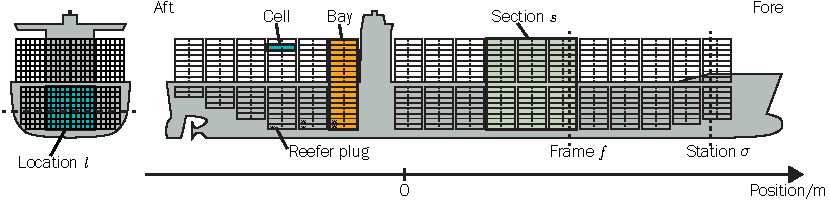
\includegraphics{vessel.pdf}
	\caption{A vessel with structures [More reefer plugs]}
	\label{fig:vessel}
\end{figure}

\paragraph{Capacities}
The vessel's capacities are given in \emph{TEU} (Twenty-foot Equivalent Units), i.e. a standard $20'$ container takes up one TEU, while a $40'$ container takes up two TEU. For each location $l$, the vessel data includes upper bounds for: the total number of TEUs ($C^\trt{TEU}_l$), 20' containers ($C^\trt{20}_l$), 40' containers ($C^\trt{40}_l$), reefer slots ($C^\trt{RS}_l$), reefer cells ($C^\trt{RC}_l$), plus separate total weight limit for $20'$ ($C^\trt{W20}_l$) and $40'$ ($C^\trt{W40}_l$) containers, respectively. The latter exist, since only $20'$ containers rest on the middle support posts of the stack it is in, while the end posts hold weight of both $20'$ and $40'$ containers. 

Limits for each tank $b$ ($\mi{Max}^\trt{t}_b$) are likewise given in the input, as well as a limit for the total weight of the vessel ($\mi{Max}^\trt{wTotal}$), including ballast water, cargo and lightship. 

\paragraph{Stress forces}
On a vessel, stress forces arise as a result of gravitation acting downwards and buoyancy acting upwards. This results in shear forces and bending moments along the longitudinal axis of the vessel, and limits on these ($\mi{Max}^\trt{sf}_f$, $\mi{Min}^\trt{sf}_f$, $\mi{Max}^\trt{bm}_f$, $\mi{Min}^\trt{bm}_f$) are given for a set of reference points along the vessel called \emph{frames} (see Figure~\ref{fig:vessel}). 
%
The buoyancy force comes from the vessel's displacement of water and hence depends on the varying (and irregular) shape of the hull and the displacement of the vessel. The area submerged in water ($A_{\sigma,d}$) is given at another set of reference points called \emph{stations} (see Figure~\ref{fig:vessel}) for a discrete set of displacement values.   

The stability requirements for the vessel is thus described by the sets $ST$ (stations) and $F$ (frames), which all are specified with a longitudinal position $(P_\sigma$, $P_f$). For modeling purposes, an (artificial) station and a frame are assumed given at the endpoinst of the vessel for which the submerged areas and limits, respectively, are 0.

Further requirements to ensure the stability of the vessel are imposed in real life and considered eg. in \cite{AlbertosThesis}, but is not considered here.

\subsection*{Standard Vessel Model}
\paragraph{Sections}
The goal of our Standard Vessel Model is to describe the various capacity- and hydrostatic constraints reasonably accurate, while abstracting away from unnecessary details relating to the irregularity of the vessel's shape and the non-coinciding reference points of tanks, bays, stations and frames. Instead, we will use bigger \emph{sections} of the vessel and their endpoints (see Figure~\ref{fig:vessel}) as the common reference for capacities and hydrostatic constraints.
 
To transform the vessel's data into a standard model, we therefore also require the set $S$ of sections given, which is divided into sections fore ($S^\trt{f}$) and sections aft ($S^\trt{a}$), as well as the partition of $L$ into sets $L_s$ for all $s\in S$, which specifies the locations that $s$ consists of. Naturally, this partition is such that all locations in the same bay belongs to the same section. Taking the minimum aft-position of the locations in $s$ and the maximum fore-position, respectively, specifies the fore position, $P^\trt{f}_s$, and aft position, $P^\trt{a}_s$, of $s$.

\paragraph{Variables}
As decision variables we use $x_{s,\tau}$ for all $s\in S$ and $\tau \in T$, which denotes the number of containers of type $\tau$ stowed in sections $s$, and $xt_s$ for all $s\in S$, which denotes the amount of ballast water in ballast tanks in section $s$. 

As an important auxiliary variable, we define $x_\tau = \sum_{s\in S} x_{s,\tau}$, the number of containers of type $\tau$ on the vessel in total, disregarding their placements. It is the relationship among these variables that we are actually interested in.  
Another important auxiliary variable is $w_s$, denoting the total weight of section $s$, everything included. Likewise the total weight, $\mi{wTotal} = \sum_{s\in S}w_s$ is used in hydrostatics constraints (see further below). 
Other auxiliary variables used to ease notation are mentioned below as necessary.

\paragraph{Location-based constraints}
For each section $s$ we define the capacity of a certain type, eg. $C^\trt{20}_s$, by summing the corresponding capacities for all locations $l\in L_s$. Naturally, we then require that the number/weight of containers of the given type in $s$ is within this limit, eg. $\sum_{\tau \in T^\trt{20}}x_{s,\tau}\leq C^\trt{20}_s$. 
This principle is applied to all the aforementioned location-based capacities.

The amount of (ballast) water in any section $s$ should not exceed the combined amount of water in the portion of each tank that lies within that section; multiplying the latter amount  of water with the density for ballast water, we get an upper bound for $xt_s$, which is then imposed as a constraint.
We also define constraints to ensure that all variables $x_{s,\tau}$ and $xt_s$ are positive and that $\mi{wTotal}\leq\mi{Max}^\trt{wTotal}$. 

\paragraph{Hydrostatic constraints}
At each station $\sigma$ the submerged area of the cross-section for a given displacement $d$ in a discrete set of values is given by the table $A_{\sigma,d}$. From this we can make an approximation of the area at $\sigma$ for any positive $d$ by linearizing it between the maximal $d$ value given in the table and a value $d_\mi{min}$ at the point where the hull does not ``curve'' too much anymore; for the cross-section given in Figure~\ref{fig:vessel} this would correspond to the displacement giving the marked water line.
We note that since our Standard Vessel Model will mainly be used for some sort of maximization of loaded cargo it is a fair assumption to make that the displacement will be above the found $d_\mi{min}$.  
The submerged area at a point $p$ between two consecutive stations $\sigma$ and $\sigma'$ for a displacement $d$ can then also be linearized as a function of the longitudinal position of $p$. 
From this we then calculate an approximation of the buoyancy of section $s$ for a given $d$ by averaging the areas between the two endpoints of $s$ and multiplying with the distance between the points; if there are stations lying within $s$, several volumes are calculated and added.
On the other hand, the downward-acting force at section $s$ is given by the weight $w_s$. For $s$, the resulting force is thus the weight of section $s$ minus the (positive) buoyancy stemming from $s$.  
  
Given a displacement $d$, the shear forces and bending moment at each section $s$'s aft endpoint is then calculated. For sections in $S^\trt{f}$ ($S^\trt{a}$) the shear force  equals the sum of resulting forces fore (aft) of the aft endpoint $P^\trt{a}_s$, while the bending moment equals the sum of resulting forces of sections $s'$ lying fore (aft) $P^\trt{a}_s$ times the distance from $P^\trt{a}_s$ to $s'$'s (longitudinal) midpoint.

To obtain upper (lower) bounds for the shear force at the sections' aft endpoints,  
we linearize the upper (lower) bound for the shear force between two consecutive frames as a function of their position. To obtain the bounds for the shear force at the aft endpoint of $s$ we then use this linearization given by the point's two closest surrounding frames. Similarly for the upper and lower bounds for the bending moment.

Hydrostatic constraints are then added to our model to ensure that the shear force and bending moment at each section's aft endpoint is within the calculated upper and lower bounds.

%\end{document}
